\documentclass[preprint,12pt]{elsarticle}
%\documentclass[12pt]{article}
\usepackage{graphicx}
%\usepackage{authblk}

\usepackage[margin=1.0in]{geometry}
\usepackage{color, colortbl}
\usepackage{hyperref}
\usepackage{float}
%\usepackage[affil-it]{authblk}

\usepackage{subcaption}
\newcommand{\note}[1]{\textcolor{blue}{#1}}
\definecolor{LightCyan}{rgb}{0.88,1,1}
\definecolor{LightRose}{rgb}{1,0.88,0.88}
\definecolor{LightGreen}{rgb}{0.88,1,0.88}

\usepackage{listings}
\usepackage{color}

\definecolor{dkgreen}{rgb}{0,0.6,0}
\definecolor{gray}{rgb}{0.5,0.5,0.5}
\definecolor{mauve}{rgb}{0.58,0,0.82}

\lstset{frame=tb,
  language=Java,
  aboveskip=3mm,
  belowskip=3mm,
  showstringspaces=false,
  columns=flexible,
  basicstyle={\small\ttfamily},
  numbers=none,
  numberstyle=\tiny\color{gray},
  keywordstyle=\color{blue},
  commentstyle=\color{dkgreen},
  stringstyle=\color{mauve},
  breaklines=true,
  breakatwhitespace=true,
  tabsize=3
}

\title{HIPO Data Format Performance Compared to ROOT}
\author[1]{Gagik Gavalian}
%\affil[1]{Jefferson Lab, Newport News, VA, USA}
% \affiliation[1]{organization={CRTC, Department of Computer Science, Old Dominion University}, city={Norfolk, VA}, country={USA}}
\address[1]{Jefferson Lab, Newport News, VA, USA}

\begin{document}
%\begin{titlepage}
\begin{abstract}
  In this paper, we present studies of the performance of High-Performance Output (HIPO)~\cite{HipoLib} data format in
  writing and reading scientific data from Nuclear Physics experiments in CLAS12~\cite{Burkert:2020akg}. The performance of
  HIPO is compared to widely used in the high-energy physics community data format of ROOT~\cite{Brun:1997pa} files.
  Our studies show that HIPO reader and writer codes in C++ and Java outperform ROOT by a significant margin.
\end{abstract}
%\end{titlepage}
\maketitle

\section{Introduction}
\indent

Modern High Energy and Nuclear Physics experiments produce an ever-increasing amount of data. This represents 
challenges in data processing categorization and monitoring. Data collected from experimental setups undergo several
iterations of processing data to produce an output that can be used for physics analysis. It is important to use a data storage 
format able to read and write a large amount of data fast. 

\section{High Performance Output Data Format}

In Nuclear Physics experiments data is stored in "event" representing one interaction of the beam with the target particle. 
Each event is a record containing variable-length collections of data structures (called banks) each representing processed 
data from different detector components. 
In CLAS12 the reconstructed particles stored in such structures are used for the final physics analysis. The event from the data 
processing stage is processed by data classifying algorithm to produce reduced outputs for each physics group containing 
different physics event topologies. In CLAS12 experiments the data selection and reduction process (called data trains) is
run on a regular basis to provide users with updated data samples to analyze. The data reduction process is primarily reading
data, categorizing a writing several data streams, and data both data reading and writing performance is important.
The High-Performance Output (HIPO) data format was developed at Jefferson Lab for CLAS12 detector data processing 
applications. It is an event-based data container with an indexed entry map that allows fast random access to any event in the file
with low latency. Two methods of compression are implemented by default for HIPO files: LZ4 and GZIP, for all the tests in this 
paper we used LZ4 compression due to its high rate of compression and decompression. 
The HIPO format is used to store raw data information from experimental data acquisition, then processed with a data processing 
application to produce final physics data for analysis in the same file format. 
CLAS12 data processing program is using Service Oriented Architecture (SOA)~\cite{Gyurjyan:2011zz} implemented in Java~\cite{Ziegler:2020gsr}. 
The reconstructed data is analyzed using a ROOT-based analysis framework (clas12root) in C++. HIPO supports C++ and Java (native) for reading files
and Python. In this paper, we test the performance of HIPO for both libraries (C++ and Java) and compare them to the performance of
ROOT Trees, which is the most commonly used data format in High Energy and Nuclear Physics community for storing and analyzing
experimental physics data.

\section{Benchmark Code}

To test the performance of each data format we used a file that contains only one data structure 
describing the particles reconstructed from experimental data. The data contains 12 columns 
with particle momentum and vertex components and some auxiliary variables such as :
particle id, charge, beta, status, and particle id $\chi^2$. Each entry contains a variable number of
rows. The test consists of reading each entry in the tree then looping through a number of particles
in each entry and calculating some quantity which involves all the columns in the bank and filling a histogram.
The size of the file in each format (HIPO and ROOT) is approximately 2GB, produced using the LZ4 
compression algorithm. 
%The code used in benchmarks:

%\begin{lstlisting}
%   auto file = TFile::Open(inputFile);
%   auto tree = file->Get<TTree>("clas12");
%   int count;
%   float  pid[1000];
%   float  px[1000];
%   ...// supressed variabbles: py,pz,vx,vy,vz,beta,charge,chi2pid
%   int16_t status[1000];
%   TBranch *br_count = nullptr;
%   TBranch *br_px = nullptr;
%   ...// supressed variabbles: py,pz,vx,vy,vz,beta,charge,chi2pid
%   TBranch *br_status = nullptr;
%   tree->SetBranchAddress("count", &count, &br_count);
%   tree->SetBranchAddress("px", px, &br_px);
%   ...// supressed variabbles,	py,pz,vx,vy,vz,beta,charge,chi2pid
%   tree->SetBranchAddress("status", status, &br_status);
%    for (decltype(nEntries) entryId = 0; entryId < nEntries; ++entryId) {
%     tree->LoadTree(entryId);
%      br_count->GetEntry(entryId);
%      br_px->GetEntry(entryId);
%      ...// supressed variabbles: py,pz,vx,vy,vz,beta,charge,chi2pid
%      br_status->GetEntry(entryId);
%      for (int i = 0; i < count; ++i) { 
%        h->Fill(
%                sqrt(px[i]*px[i] + py[i]*py[i] + pz[i]*pz[i])*sqrt(vx[i]*vx[i]+vy[i]*vy[i]+vz[i]*vz[i])
%                + vt[i] + pid[i]*beta[i]*chi2pid[i]+status[i] - charge[i]);
%      }
%}
%\end{lstlisting}

The listing above shows ROOT code used to analyze the data using an improved implementation of 
ROOT Tree~\cite{Blomer:2020usr} provided to the authors through private communications.
The code was translated to Java (almost exactly) to benchmark the performance of the HIPO/Java library and
was tested using GraalVM 17 platform.
The benchmarks were run on different platforms including M1, AMD, and Intel/Xeon architectures.
We also run benchmarks in two different scenarios where the data was read from NFS disks (AMD and Intel/Xeon tests)
as well as reading the data from the local SSD hard drive (all MacBook tests). Several runs were performed with a warmup cycle,
then an average of 10 tests was taken to produce comparative plots.

%\begin{verbatim}
%\end{verbatim}

\section{Reading Benchmarks}
\indent

To benchmark file reading performance we used a file from production data that was filtered to contain
only one structure (bank) that contains information on reconstructed particles in the CLAS12 detector
containing $ 7 M$ events and a size of 2.1 Gb. The HIPO file was converted to a ROOT file using code 
provided by the ROOT team and analyses are run using the code described in the "Benchmark Code" section. 
The benchmark is run on different platforms and different environments to emulate standard everyday data 
processing scenarios. The platforms used are:

\begin{itemize}
\item MacBook Pro 16, Apple M1 Max (reading from SSD)
\item AMD EPYC 7502 32-Core Processor (NFS mounted luster)
\item Intel(R) Xeon(R) CPU E5-2697A v4 @ 2.60GHz (NFS mounted luster)
%\item Macbook Intel i9 2018 (reading from SSD)
\end{itemize}

On MacBook computers, the data is read from a local SSD drive.
The AMD and Intel/Xeon machines used in these benchmarks are part of the Jlab computing cluster 
and the data is read from NFS-mounted disks. The results of benchmarks are shown in Figure~\ref{benchmark:read},
where the execution time for each benchmark is shown in seconds.

 \begin{figure}[!h]
\begin{center}
  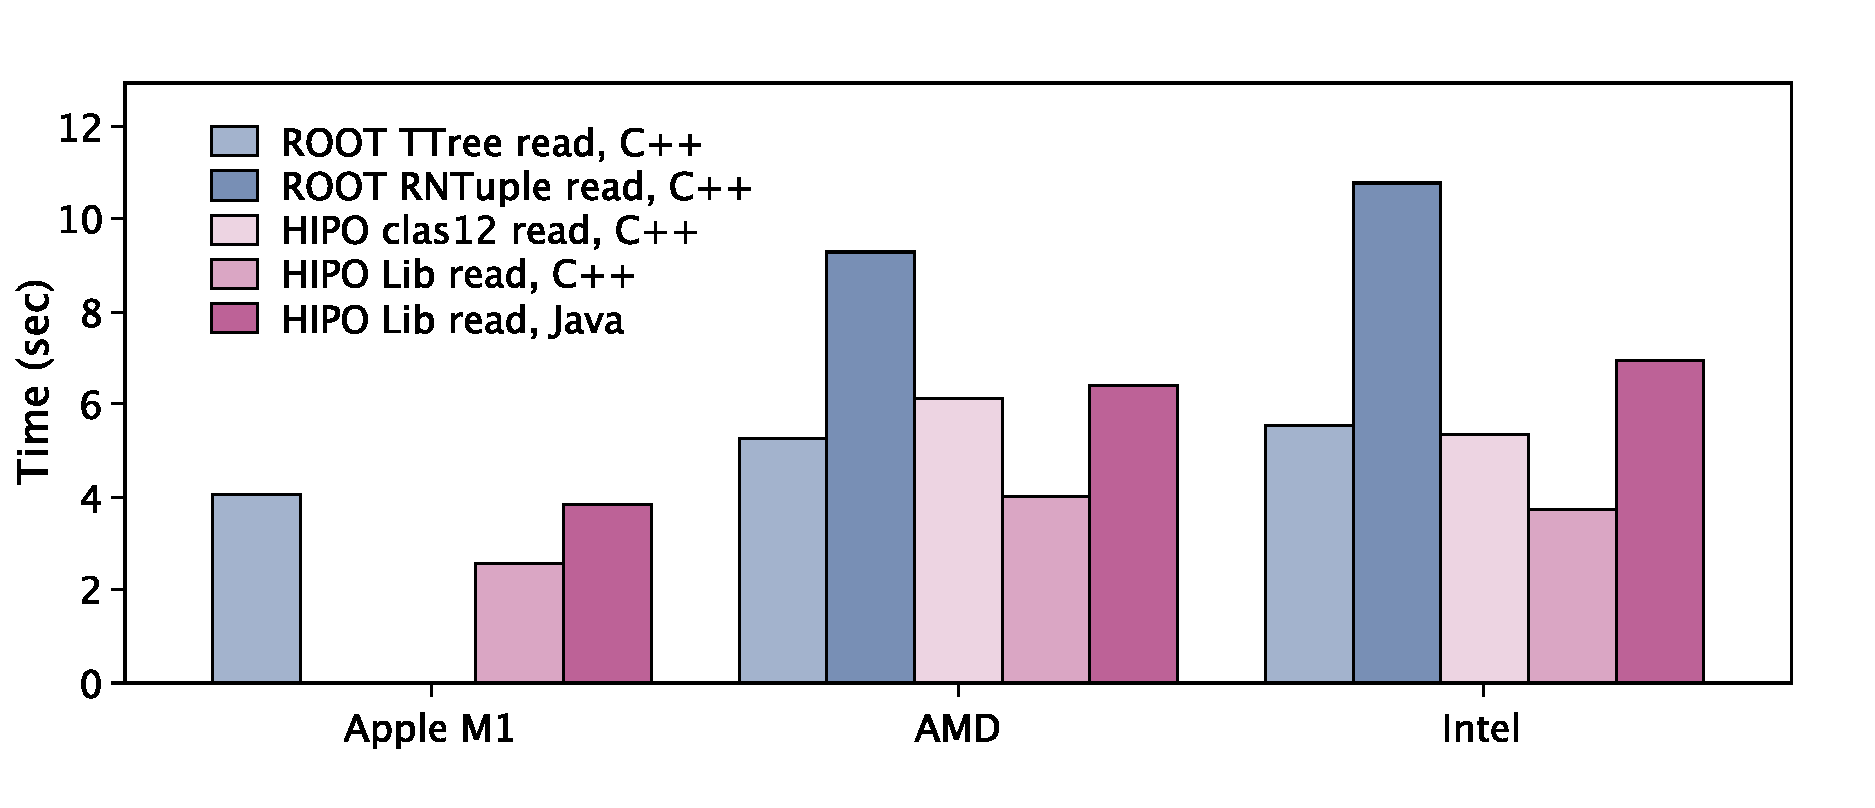
\includegraphics[width=5.0in]{bench_root_vs_hipo_read.pdf}
 \caption { Reading times for ROOT and HIPO compared for different platforms for C++ and Java. RNTuple is used for ROOT with LZ4 compression.}
 \label{benchmark:read}
 \end{center}
 \end{figure}

Few observations can be made from the Figure. The analyses in Java are always faster than code running in C++ using ROOT I/O. 
The HIPO C++ library outperforms ROOT I/O significantly, peculiarly the difference in performance is architecture-dependent. 
On M1 and AMD architecture the HIPO is about 25\%-30\% faster than ROOT, on Intel architecture the ROOT is more than twice slower.
If we consider AMD and Intel tests are done in the same environment of Jlab computer cluster in the same conditions of reading the files from NFS 
disks, it's surprising that HIPO performance is similar ($\pm 2\%$) while the ROOT I/O performance changes dramatically (almost twice) going 
from AMD to Intel Xeon. Interestingly Java library also performs the same on AMD and Intel architectures. These results are very surprising and 
hard to explain.

 \section{Writing Benchmarks}

The writing speed of the data format is important in different workflows of the data analysis process, especially in I/O bound workflows.
In CLAS12 we frequently process the data through data "trains", where we create different data samples, depending on the reconstructed event topology,
for different experimental groups to analyze. The entire reconstructed data set is processed and several (typically of the order of 14-18) separate data sets 
are written to the disk. In these kinds of applications, the data writing speed is also important since there is very little processing done by "trains" other
than checking if the event matches some topology criteria and the majority of processing time is spent on reading and writing.

We also run some tests to compare the performance of the ROOT I/O against HIPO running in C++ and Java. The results can be 
seen in Figure~\ref{benchmark:write}.

  \begin{figure}[!h]
\begin{center}
  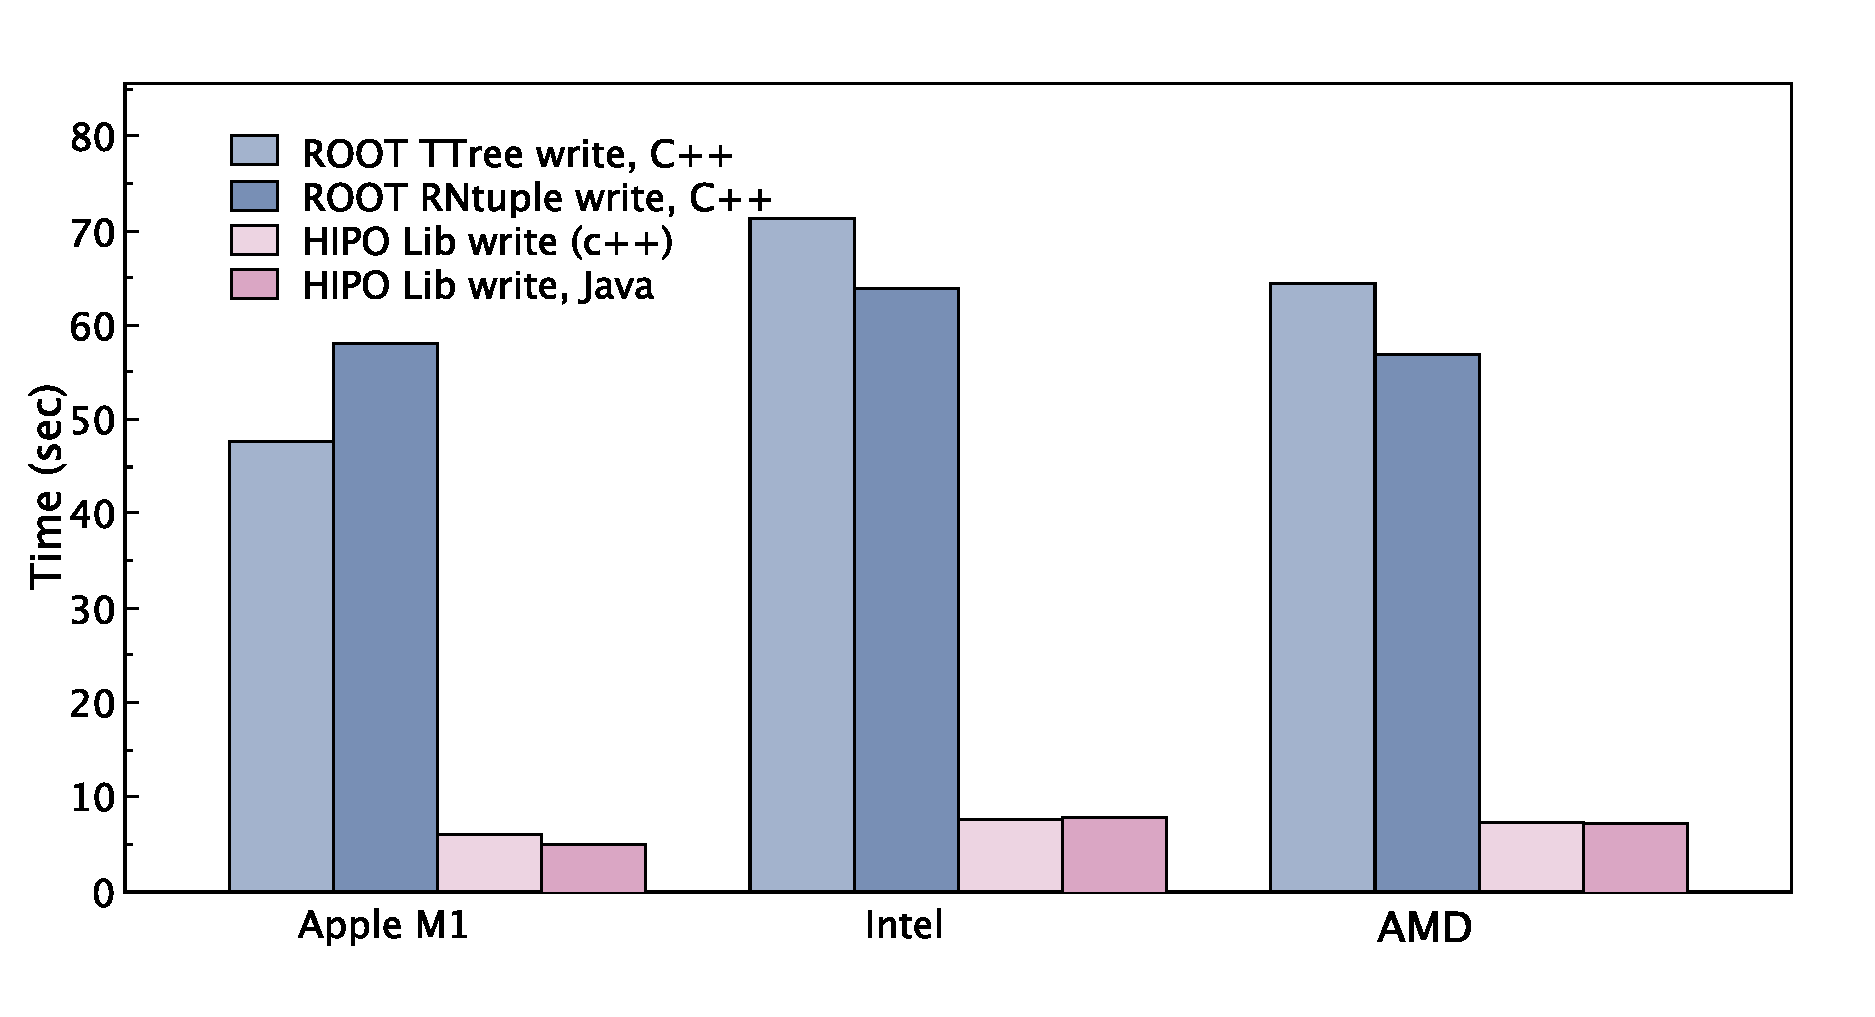
\includegraphics[width=5.0in]{bench_root_vs_hipo_write.pdf}
 \caption { Writing times for ROOT and HIPO compared for different platforms for C++ and Java. RNTuple is used for ROOT with LZ4 compression.}
 \label{benchmark:write}
 \end{center}
  \end{figure}
  
The results show that the MacBook M1 has the best writing speeds due to its very fast SSD. However, in all of the tests
HIPO C++ and HIPO Java writers outperform ROOT writers significantly. The surprise of this benchmark is that the writing 
speeds of ROOT files on AMD and Intel Xeon architectures are not very different, as it was for reading speeds.
Both data formats use same LZ4 compression algorithms, and in general writing speed will depend on level of compression requested from the  library. For both samples we used highest level of compression and we end up similar file size for both data formats, ROOT file being slightly lagrger 2,119 MB vs 2,033 MB in HiPO data format. 

%\section{CLAS12 ROOT Tree Implementation}
%In the previous sections, the performance of the ROOT data format is shown for the new ROOT tree reader. The legacy code used in 
%CLAS12 data analysis the reconstructed data is converted into a ROOT tree using \texttt{std::vector} objects for each column of the particle bank.
%The same benchmarks are run on the files produced by CLAS12  ROOT converter and times are measured for writing files and reading the 
%files and doing the analysis described in the Benchmark section. The results are shown in Figure~\ref{benchmark:root6}.

%  \begin{figure}[!ht]
%\begin{center}
%  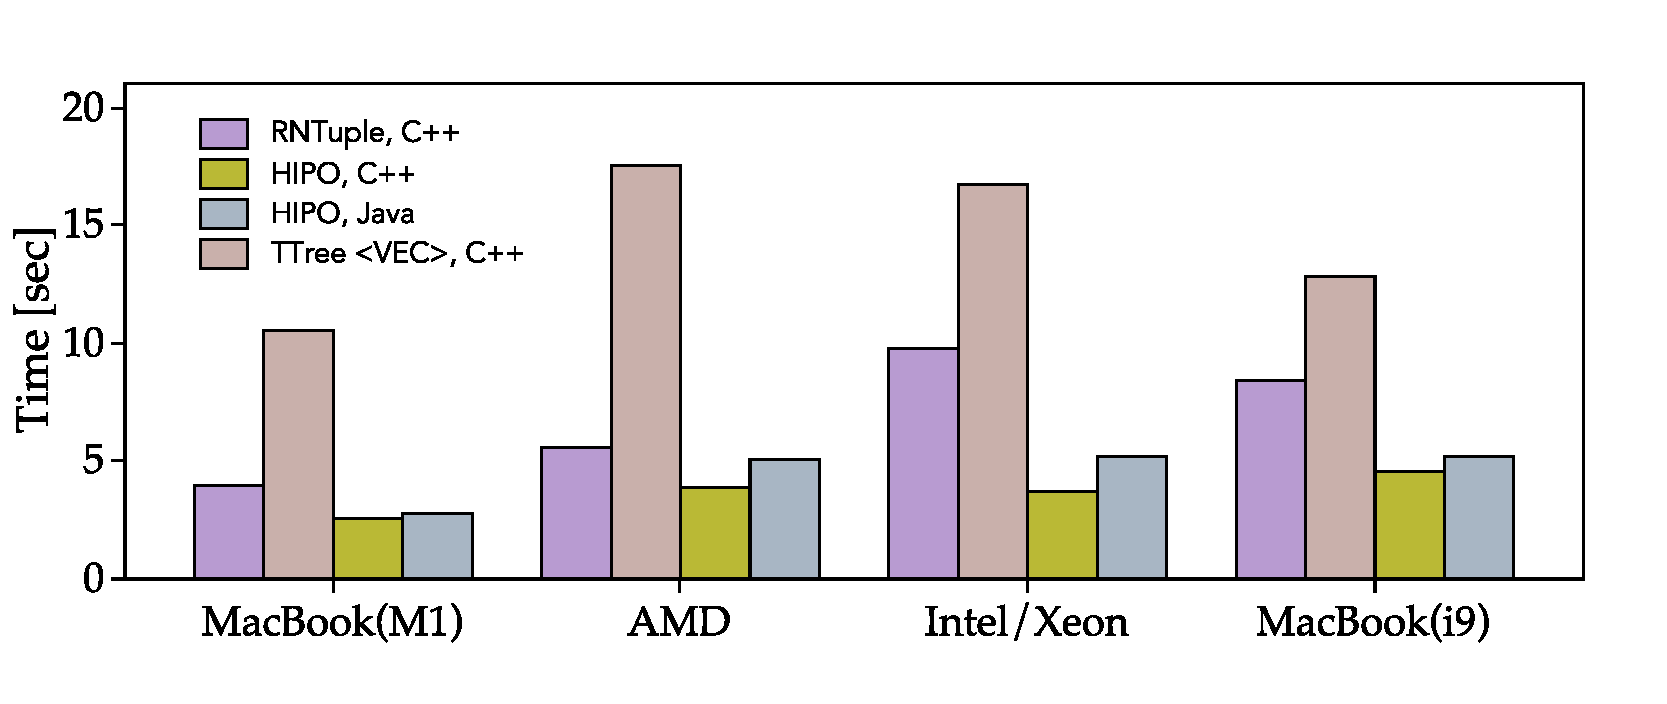
\includegraphics[width=5.0in]{root6_vs_hipo_read.pdf}
%    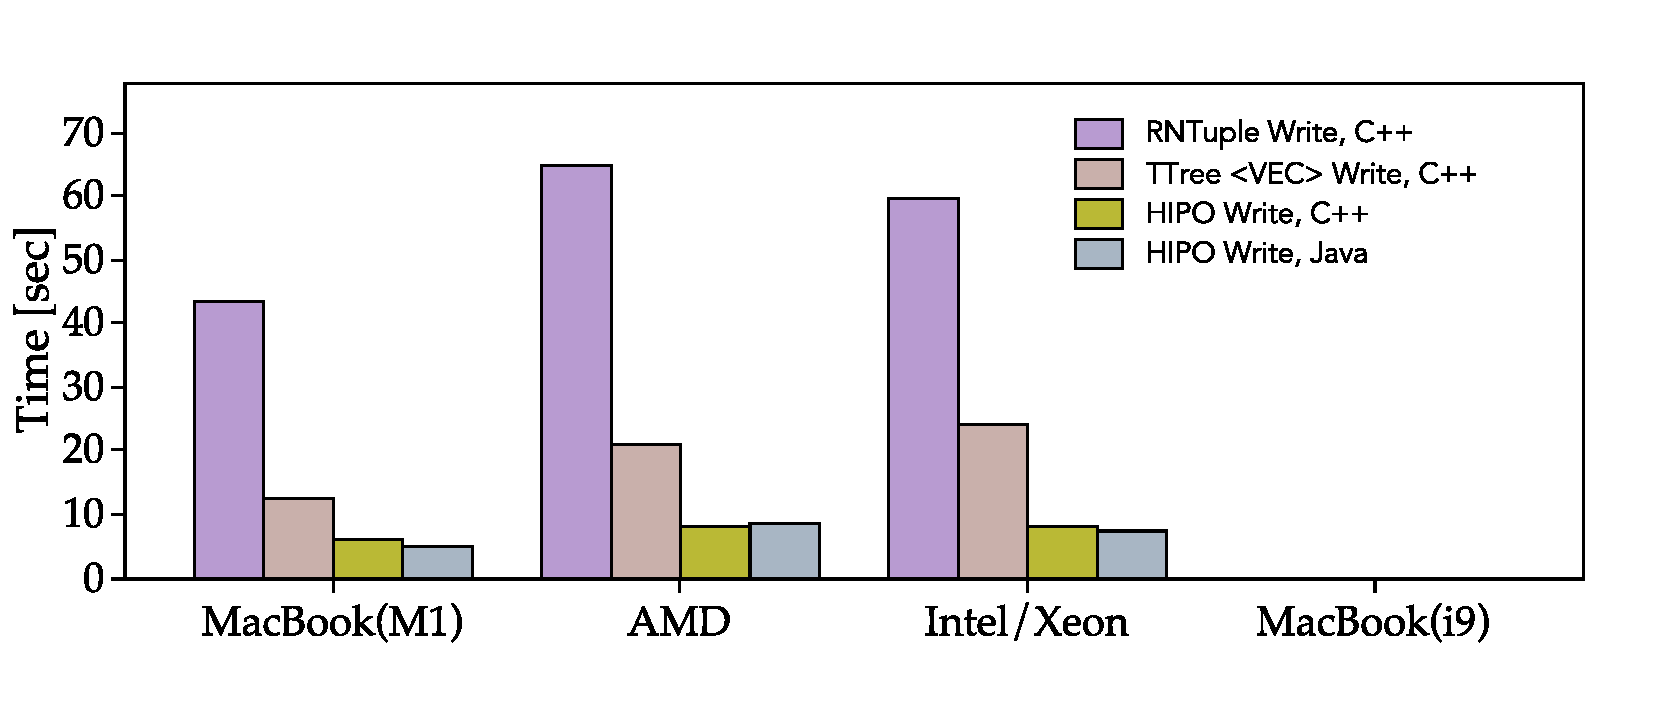
\includegraphics[width=5.0in]{root6_vs_hipo_write.pdf} 
% \caption { Reading and Writing benchmarks for ROOT and HIPO using C++ and Java libraries. The ROOT includes benchmarks with new TTreeReader as well as 
 %tree produced using old TTree with \texttt{std::vector} for the leaves of each bank.}
 %\label{benchmark:root6}
 %\end{center}
 % \end{figure}
  
  %It is apparent that the new ROOT RNTuple implementation performs significantly better in reading benchmarks, however  the \texttt{std::vector} 
  %implementation does write files significantly faster. What is perplexing is that the legacy TTree implementation does not exhibit discernible architecture 
  %dependence in reading the tree for AMD and Intel, as shown in Figure~\ref{benchmark:root6}, which was the case for RNTuple implementation. 
  %The TTree CLAS12 implementation is significantly faster in writing the data (more than twice), while significantly slower in reading the data.

 \section{Discussion}
 
 In this article, we tested the analysis performance when reading data from the ROOT tree and HIPO data format. 
 It was shown that HIPO outperforms ROOT on every tested platform and due to ROOT Tree architecture dependence 
 on Intel architecture, the difference in performance is almost double. The writing tests show a significant (5-7 times) difference in the file writing times. 
 Moreover, analysis done in Java using the Java implementation of HIPO data format outperformed analysis done using ROOT data format on all platforms
 and in all ROOT tree implementations. Writing files in Java is also significantly faster than writing ROOT trees. 
 At the early stages of CLAS12 software development, the data was converted to ROOT for final analysis, which leads to significant 
 empty computation cycles, and leads to data structures that are slower to process. With the development of CLAS12ROOT package (in C++)
 the HIPO files can be easily read into the ROOT environment and analyzed using data analysis and visualization tools available in ROOT.
 
 
\newpage
\bibliography{references}
\bibliographystyle{ieeetr}


\end{document}
